\section{Market Definition}
%Smart cities have the potential to benefit communities and individuals in a variety of applications across health, transportation, education, government, energy, and power and water. Implemented correctly, smart city applications can reduce costs, simplify services and offer a sustainable solution. \cite{smart_city_application_needs} 
%
%\begin{figure}[ht]
%	\centering
%	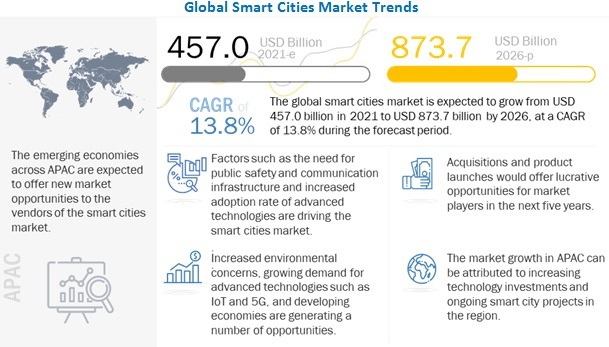
\includegraphics[width=.85\textwidth]{/02market_research/smart_cities_market}
%	\caption{Global smart cities market trends.}
%	\label{fig:smart_city_growth}
%\end{figure}
%
%\clearpage
%
%As one can see, in figure \ref{fig:smart_city_growth}, according to MarketsandMarkets \cite{smart_cities_market} global smart cities market is expected to grow from USD 457 billion in 2021 to USD 873.7 billion by 2026, at a \ac{cagr} of 13.8\%, during the forecast period. Growing urbanization, need for efficient management and utilization of resources, and also the increasing demand for a healthy environment with efficient energy consumption are expected to be the major factors driving the growth of the smart cities market.

As figure \ref{fig:smart_cities_sols} shows, there are various applications of \ac{iot} technology for smart cities. In this project it will be created a solution that comprises Smart Lighting management and Smart Parking.

\begin{figure}[ht]
	\centering
	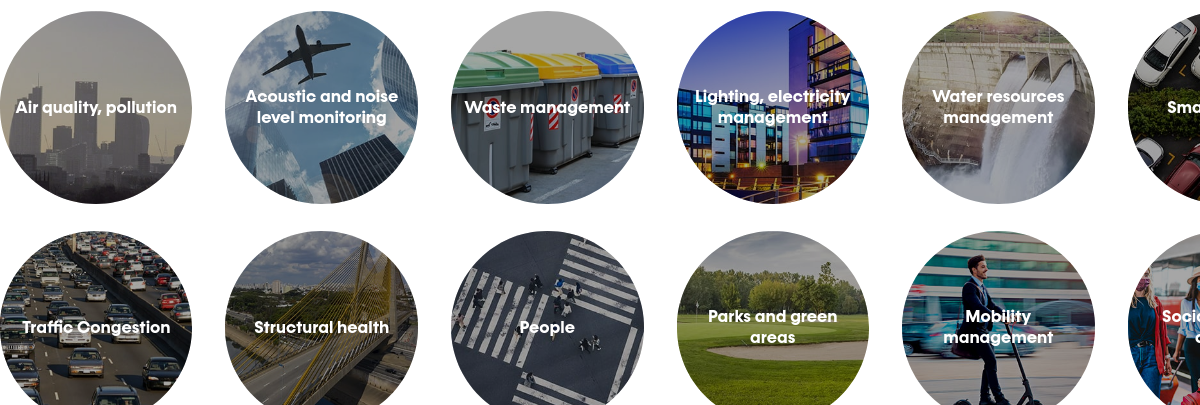
\includegraphics[width=1\textwidth]{/02market_research/applications_for_smart_cities}
	\caption{Applications of \ac{iot} technology for Smart Cities. \cite{smart_cities_solutions}}
	\label{fig:smart_cities_sols}
\end{figure}

The \ac{iot} starts with connectivity, but since it is a widely diverse and multifaceted realm, one certainly cannot find a one-size-fits-all communication solution. Next, one can identify these common types of \ac{iot} wireless technologies, through mesh and star topologies:

\begin{itemize}
	\item \textbf{LoRaWAN} (LoRa from "long range") is a \ac{lpwan} specification that targets key requirements of \ac{iot}, such as secure bi-directional communication. LoRaWAN network architecture is deployed in a star-of-stars topology in which gateways relay messages between end-devices and a central network server. The gateways are connected to the network server via standard IP connections and act as a transparent bridge, simply converting \ac{rf} packets to IP packets and vice versa. The wireless communication takes advantage of the Long Range characteristics of the LoRa physical layer, allowing a single-hop link between the end-device and one or many gateways. \cite{lorawan}
	
	\item \textbf{Wi-SUN} (\ac{ieee} standard 802.15.4g) is a \ac{rf} mesh communication technology, which enables large-scale outdoor IoT networks including applications such as asset management, environmental monitoring, agriculture, structural health monitoring and much more. \cite{wi_sun} Using the same \ac{ieee} standard, there is also \textbf{ZigBee}, a short-range, low-power, commonly deployed in mesh topology to extend coverage by relaying sensor data over multiple sensor nodes. \cite{zigbee}
	
	\item \textbf{Sigfox} is a cellular style communication technology that provides low power, low data rate and low communication costs for \ac{iot} applications. Sigfox employs \ac{unb} technology, which enables very low transmitter power levels to be used while still being able to maintain a robust data connection, using unlicensed \ac{ism} radio bands. The simple and easy to rollout star-based cell infrastructure has encouraged its current extended worldwide availability. \cite{sigfox}
	
	\item \textbf{\ac{nb-iot}} is a carrier-grade \ac{rf}, narrowband communication technology, specially designed for the \ac{iot}. It connects devices more simply and effciently on already established mobile networks, and handles small amounts of infrequent 2-way data, securely and reliably. The special focus of this standard is on very low power consumption, excellent penetration coverage and lower component costs, deployed in GSM and LTE regulated frequencies. \cite{nb-iot}
	
	\item \textbf{\ac{lte-m}} is a \ac{lpwa} technology standard published by 3GPP. It supports \ac{iot} through lower device complexity and extended coverage, while allowing the reuse of the LTE installed base. Supported by all major mobile equipment, chipset and module manufacturers, \ac{lte-m} networks will co-exist with 2G, 3G, and 4G mobile networks and benefit from all the security and privacy features of carrier-grade networks. 
	\cite{lte-m}
\end{itemize}

\subsection{Smart Lighting}
Smart Street lighting is a rapidly growing lighting market, with an expected \ac{cagr} of 20.4 \% until 2026 \cite{smart_light_market}, implementing a smart management of public lighting to optimize energy consumption according to lighting needs. This is boosted by regulatory policies that encourage energy efficiency, \ac{iot} convergence and the drop of \ac{led} prices. This new concept of smart light post is also growing, implementing not only the smart management of street lights, but also features that go from basic \ac{led} replacement control, to traffic and video monitoring, environmental monitoring, and others. 

\subsubsection{FLASHNET - inteliLIGHT}
FLASHNET is a company focused on developing intelligent systems for smarter cities and better infrastructures and have created a solution that provides the right amount of light where and when needed to lighten the streets, the inteliLIGHT. \cite{inteli_light} Using the existing infrastructure, this solution saves money and transforms the existing distribution level network into an intelligent infrastructure of the future.

\clearpage
\begin{figure}[ht]
	\centering
	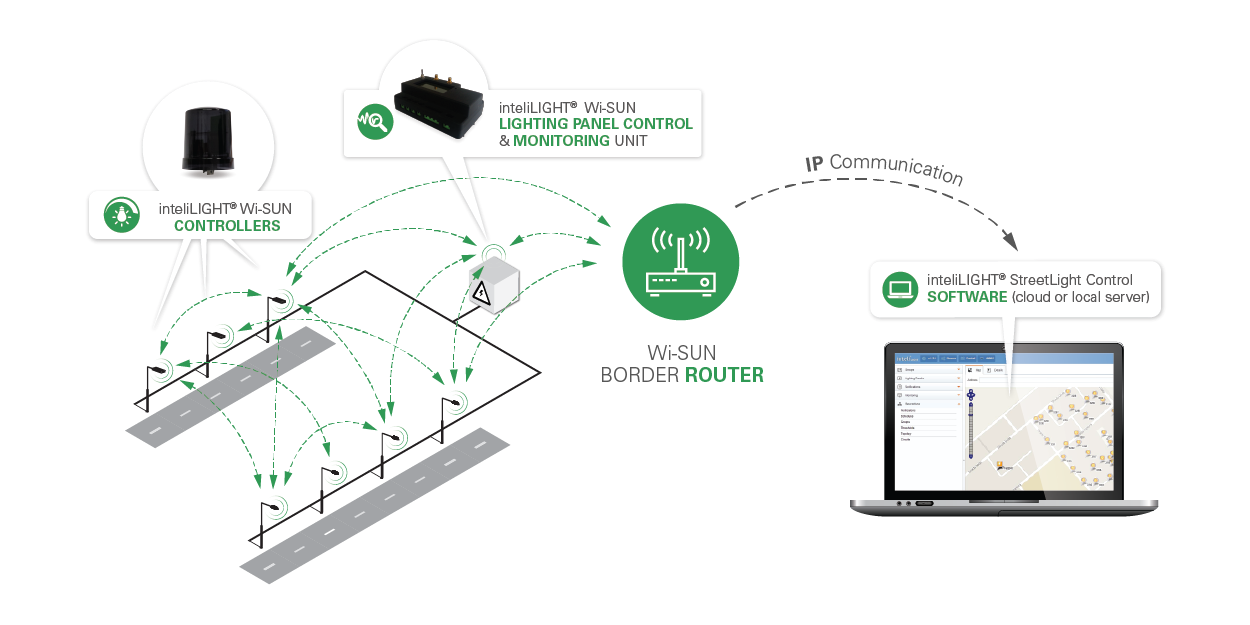
\includegraphics[width=0.85\textwidth]{/02market_research/intelilight}
	\caption{inteliLIGHT Communication Technology.}
	\label{fig:intelilight}
\end{figure}

In figure \ref{fig:intelilight} it is presented one of the many communication technologies that inteliLIGHT can provide in their smart street light solution. In this case, it is shown the use of Wi-SUN, a \ac{rf} mesh street lighting communication technology.
Furthermore, the system is integrated with major \ac{iot} platforms and provides \ac{api} connectivity with City Management applications, ensuring compatibility with existing smart lighting and smart city initiatives.

\subsubsection{Telensa - PLANet}
Nowadays, Telensa is the market share leader in smart street lighting with more than ten years of experience.\cite{telensa_solutions} PLANet is connected street lighting system that consists of wireless control nodes, an \ac{unb} wireless network and a Central Management System, as seen in figure \ref{fig:telensa}. This system reduces energy and maintenance costs associated with street lighting and also improves quality of maintenance through automatic fault reporting.
\clearpage
\begin{figure}[ht]
	\centering
	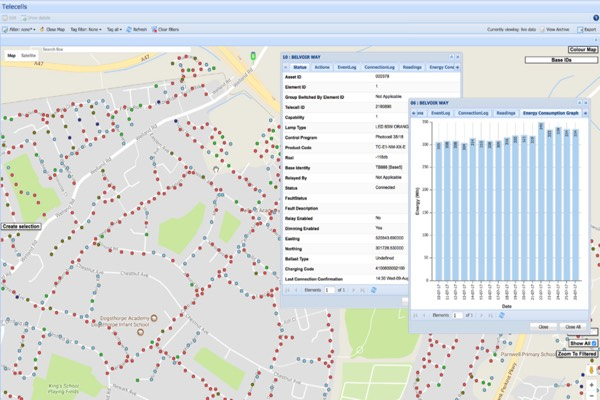
\includegraphics[width=0.8\textwidth]{/02market_research/telensa}
	\caption{Telecells - PLANet's Central Management System.}
	\label{fig:telensa}
\end{figure}

\subsection{Smart Parking}
Smart parking, through the monitoring of parking spaces availability in the city, is also a growing market, expected to grow with a \ac{cagr} of 17.85\% in the forecast period of 2021 to 2028.\cite{smart_parking_market} The rise in investment in building driverless vehicles and an increase in the government’s initiative in building smart cities across the globe, along with the demand and adoption of \ac{iot} technology, are the main driving factors for the growth of smart parking market.

\subsubsection{intuVision - intuVision VA Parking}
Regarding only to the detection of available parking spaces, there is a solution, by intuVision, named intuVision VA Parking, which provides parking lot analytics to determine vehicle count and security, and monitor parking space availability at all times, both for cities and for private parking lots, as one can see in the figure \ref{fig:intuvision}.\cite{parking}

\begin{figure}[ht]
	\centering
	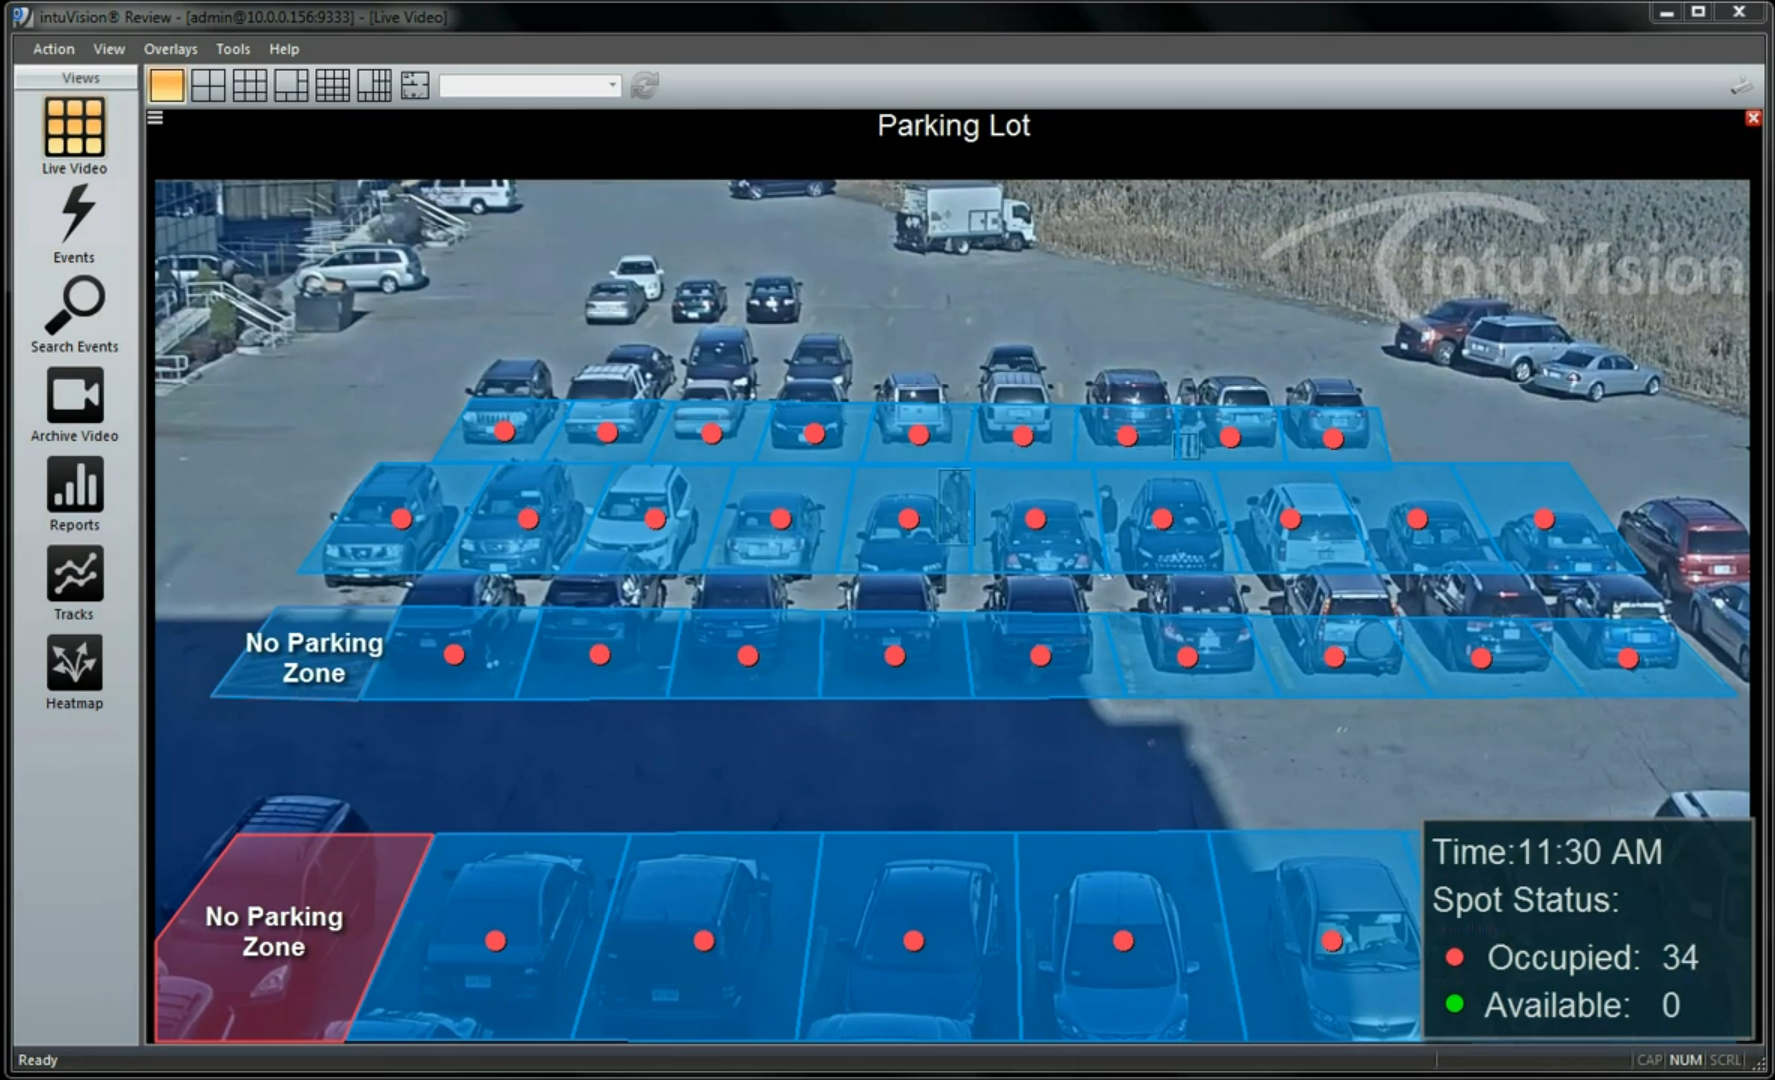
\includegraphics[width=0.8\textwidth]{/02market_research/intuvision}
	\caption{intuVision Parking Lot Demonstration.}
	\label{fig:intuvision}
\end{figure}

\section{Why choose our product}
This product aims to decrease power consumption associated with the traditional street light network, and also, using that infrastructure, contribute to the development of a smart city, detecting available parking spaces in the streets. This street lighting solution can be used in residential areas, public spaces or a large outdoor parking lot, feasible of being installed in existent lamp posts, requiring minimum changes to the original infrastructure. Although in this project it is not implemented, aside the parking spaces availability detection, this product can have the ability to monitor and to process various areas of interest using the camera built in, like for example, security purposes.
